\documentclass{report}
\setlength{\parskip}{\baselineskip}%
\usepackage{amsmath}
\usepackage{amsfonts,stmaryrd,amssymb} % Math packages

\usepackage{enumerate} % Custom item numbers for enumerations
\usepackage{fontawesome}
\usepackage{setspace}
\usepackage{hyperref}
\usepackage{enumitem}
\usepackage{multicol}
\usepackage{xhfill}
\usepackage[p,osf]{cochineal}
\usepackage[scale=.95,type1]{cabin}
\usepackage[cochineal,bigdelims,cmintegrals,vvarbb]{newtxmath}
\usepackage[zerostyle=c,scaled=.94]{newtxtt}
\usepackage[cal=boondoxo]{mathalfa}
\usepackage[export]{adjustbox}
\usepackage{vwcol}  
\usepackage{fancyhdr}
\DeclareSymbolFont{yhlargesymbols}{OMX}{yhex}{m}{n}
\DeclareMathAccent{\wideparen}{\mathord}{yhlargesymbols}{"F3}

\hypersetup{
	colorlinks=false,
	linkcolor=black,
	filecolor=black,      
	urlcolor=black,
	pdftitle={Overleaf Example},
	pdfpagemode=FullScreen,
	urlbordercolor=white,
}

\urlstyle{same}


	
\newenvironment{cequation}{
	\makeatletter
	\setbool{@fleqn}{false}
	\makeatother
	\begin{equation*}
		}{\end{equation*}}
		
\newcommand{\sol}{\noindent\textbf{Solution:} }
%----------------------------------------------------------------------------------------

\newcommand{\exercise}[1]{%
	\subsection*{\faPencil\ \ Exercise #1\hspace{0.5em}\xrfill[0.175\baselineskip]{1pt}}
}

\newcommand{\practice}[1]{%
	\subsection*{\faFlag\ \ Practice #1\hspace{0.5em}\xrfill[0.175\baselineskip]{1pt}}
}

\newcommand{\revision}[1]{%
	\section*{\faGears\ \ Revision Exercise #1\hspace{0.5em}\xrfill[0.175\baselineskip]{1pt}}
}

\usepackage[ruled]{algorithm2e} % Algorithms

\usepackage[framemethod=tikz]{mdframed} % Allows defining custom boxed/framed environments

\usepackage{listings} % File listings, with syntax highlighting
\lstset{
	basicstyle=\ttfamily, % Typeset listings in monospace font
}

%----------------------------------------------------------------------------------------
%	DOCUMENT MARGINS
%----------------------------------------------------------------------------------------

\usepackage{geometry} % Required for adjusting page dimensions and margins

\geometry{
	paper=a4paper, % Paper size, change to letterpaper for US letter size
	top=2.5cm, % Top margin
	bottom=3cm, % Bottom margin
	left=2.5cm, % Left margin
	right=2.5cm, % Right margin
	headheight=14pt, % Header height
	footskip=1.5cm, % Space from the bottom margin to the baseline of the footer
	headsep=1.2cm, % Space from the top margin to the baseline of the header
	%showframe, % Uncomment to show how the type block is set on the page
}

%----------------------------------------------------------------------------------------
%	FONTS
%----------------------------------------------------------------------------------------

\usepackage[utf8]{inputenc} % Required for inputting international characters
\usepackage[T1]{fontenc} % Output font encoding for international characters

%----------------------------------------------------------------------------------------
%	COMMAND LINE ENVIRONMENT
%----------------------------------------------------------------------------------------

% Usage:
% \begin{commandline}
%	\begin{verbatim}
%		$ ls
%		
%		Applications	Desktop	...
%	\end{verbatim}
% \end{commandline}

\mdfdefinestyle{commandline}{
	leftmargin=10pt,
	rightmargin=10pt,
	innerleftmargin=15pt,
	middlelinecolor=black!50!white,
	middlelinewidth=2pt,
	frametitlerule=false,
	backgroundcolor=black!5!white,
	frametitle={Command Line},
	frametitlefont={\normalfont\sffamily\color{white}\hspace{-1em}},
	frametitlebackgroundcolor=black!50!white,
	nobreak,
}

% Define a custom environment for command-line snapshots
\newenvironment{commandline}{
	\medskip
	\begin{mdframed}[style=commandline]
		}{
	\end{mdframed}
	\medskip
}

%----------------------------------------------------------------------------------------
%	FILE CONTENTS ENVIRONMENT
%----------------------------------------------------------------------------------------

% Usage:
% \begin{file}[optional filename, defaults to "File"]
%	File contents, for example, with a listings environment
% \end{file}

\mdfdefinestyle{file}{
	innertopmargin=1.6\baselineskip,
	innerbottommargin=0.8\baselineskip,
	topline=false, bottomline=false,
	leftline=false, rightline=false,
	leftmargin=2cm,
	rightmargin=2cm,
	singleextra={%
		\draw[fill=black!10!white](P)++(0,-1.2em)rectangle(P-|O);
		\node[anchor=north west]
		at(P-|O){\ttfamily\mdfilename};
		%
		\def\l{3em}
		\draw(O-|P)++(-\l,0)--++(\l,\l)--(P)--(P-|O)--(O)--cycle;
		\draw(O-|P)++(-\l,0)--++(0,\l)--++(\l,0);
	},
	nobreak,
}

% Define a custom environment for file contents
\newenvironment{file}[1][File]{ % Set the default filename to "File"
	\medskip
	\newcommand{\mdfilename}{#1}
	\begin{mdframed}[style=file]
		}{
	\end{mdframed}
	\medskip
}

%----------------------------------------------------------------------------------------
%	NUMBERED QUESTIONS ENVIRONMENT
%----------------------------------------------------------------------------------------

% Usage:
% \begin{question}[optional title]
%	Question contents
% \end{question}

\mdfdefinestyle{question}{
	innertopmargin=1.2\baselineskip,
	innerbottommargin=0.8\baselineskip,
	roundcorner=5pt,
	nobreak,
	singleextra={%
		\draw(P-|O)node[xshift=1em,anchor=west,fill=white,draw,rounded corners=3pt]{%
			\faCaretRight\ \textbf{Example \theQuestion\questionTitle}};
	},
}

\newcounter{Question} % Stores the current question number that gets iterated with each new question

% Define a custom environment for numbered questions
\newenvironment{question}[1][\unskip]{
	\bigskip
	\stepcounter{Question}
	\newcommand{\questionTitle}{~#1}
	\begin{mdframed}[style=question]
		}{
	\end{mdframed}
	\medskip
}

%----------------------------------------------------------------------------------------
%	SOLUTIONS ENVIRONMENT
%----------------------------------------------------------------------------------------

% Usage:
% \begin{solution}
%	Solution contents
% \end{solution}

\mdfdefinestyle{solution}{
	innertopmargin=1.2\baselineskip,
	innerbottommargin=0.8\baselineskip,
	roundcorner=5pt,
	nobreak,
	singleextra={%
		\draw(P-|O)node[xshift=1em,anchor=west,fill=white,draw,rounded corners=5pt]{解};
	},
}

% Define a custom environment for solutions
\newenvironment{solution}{
	\begin{mdframed}[style=solution]
		}{
	\end{mdframed}
}

%----------------------------------------------------------------------------------------
%	WARNING TEXT ENVIRONMENT
%----------------------------------------------------------------------------------------

% Usage:
% \begin{warn}[optional title, defaults to "Warning:"]
%	Contents
% \end{warn}

\mdfdefinestyle{warning}{
	topline=false, bottomline=false,
	leftline=false, rightline=false,
	nobreak,
	singleextra={%
		\draw(P-|O)++(-0.5em,0)node(tmp1){};
		\draw(P-|O)++(0.5em,0)node(tmp2){};
		\fill[black,rotate around={45:(P-|O)}](tmp1)rectangle(tmp2);
		\node at(P-|O){\color{white}\scriptsize\bf !};
		\draw[very thick](P-|O)++(0,-1em)--(O);%--(O-|P);
	}
}

% Define a custom environment for warning text
\newenvironment{warn}[1][Warning:]{ % Set the default warning to "Warning:"
	\medskip
	\begin{mdframed}[style=warning]
		\noindent{\textbf{#1}}
		}{
	\end{mdframed}
	\vspace{-0.5cm}
}

%----------------------------------------------------------------------------------------
%	INFORMATION ENVIRONMENT
%----------------------------------------------------------------------------------------

% Usage:
% \begin{info}[optional title, defaults to "Info:"]
% 	contents
% 	\end{info}

\mdfdefinestyle{info}{%
	topline=false, bottomline=false,
	leftline=false, rightline=false,
	nobreak,
	singleextra={%
		\fill[black](P-|O)circle[radius=0.6em];
		\node at(P-|O){\color{white}\scriptsize\bf \faInfo};
		\draw[very thick](P-|O)++(0,-0.8em)--(O);%--(O-|P);
	}
}

% Define a custom environment for information
\newenvironment{info}[1][Info:]{ % Set the default title to "Info:"
	\medskip
	\begin{mdframed}[style=info]
		\noindent{\textbf{#1}}
		}{
	\end{mdframed}
	\vspace{-0.5cm}
	
}

\mdfdefinestyle{explore}{%
	topline=false, bottomline=false,
	leftline=false, rightline=false,
	nobreak,
	singleextra={%
		\fill[black](P-|O)circle[radius=0.6em];
		\node at(P-|O){\color{white}\scriptsize\bf \faFlask};
		\draw[very thick](P-|O)++(0,-0.8em)--(O);%--(O-|P);
	}
}

% Define a custom environment for warning text
\newenvironment{explore}[1][Exploration Activity:]{ % Set the default warning to "Warning:"
	\medskip
	\begin{mdframed}[style=explore]
		\noindent{\large\textbf{#1}}
		}{
	\end{mdframed}
	\vspace{-0.5cm}
}

\mdfdefinestyle{think}{%
	topline=false, bottomline=false,
	leftline=false, rightline=false,
	nobreak,
	singleextra={%
		\fill[black](P-|O)circle[radius=0.6em];
		\node at(P-|O){\color{white}\scriptsize\bf \faQuestion};
		\draw[very thick](P-|O)++(0,-0.8em)--(O);%--(O-|P);
	}
}

% Define a custom environment for warning text
\newenvironment{think}[1][Think about It:]{ % Set the default warning to "Warning:"
	\medskip
	\begin{mdframed}[style=think]
		\noindent{\large\textbf{#1}}
		}{
	\end{mdframed}
	\vspace{-0.5cm}
}



\usepackage{setspace}
\usepackage{hyperref}
\usepackage{enumitem}
\usepackage{multicol}
\usepackage{xhfill}
\usepackage[p,osf]{cochineal}
\usepackage[scale=.95,type1]{cabin}
\usepackage[cochineal,bigdelims,cmintegrals,vvarbb]{newtxmath}
\usepackage[zerostyle=c,scaled=.94]{newtxtt}
\usepackage[cal=boondoxo]{mathalfa}

\hypersetup{
    colorlinks=false,
    linkcolor=black,
    filecolor=black,      
    urlcolor=black,
    pdftitle={Overleaf Example},
    pdfpagemode=FullScreen,
    urlbordercolor=white,
    }

    \urlstyle{same}

\newenvironment{cequation}{
    \makeatletter
    \setbool{@fleqn}{false}
    \makeatother
    \begin{equation*}
        }{\end{equation*}}

\newcommand{\sol}{\noindent\textbf{Solution:} }
%----------------------------------------------------------------------------------------

\begin{document}
\onehalfspacing
\setcounter{chapter}{7}

\chapter{Degree and Radian}

\section{Concept and Measurement of Arbitrary Angle}

\subsection*{Arbitrary Angle}

Back in junior high, we learned that the angle is the geometric object formed by rays from the same endpoint. As shown in the figure below, whether it is from ray $OA$ to ray $OB$, or from ray $OA$ to ray $OC$, the angle can be measured as $30^\circ$.

\begin{center}
    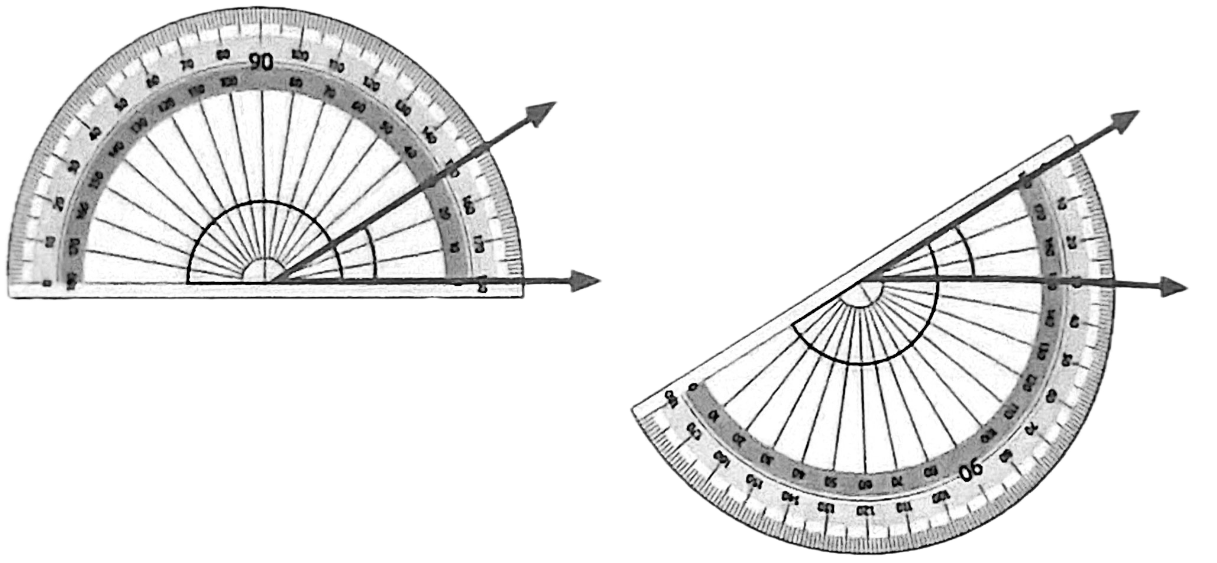
\includegraphics[scale=0.21]{assets/8-1.png}
\end{center}
\vspace{-1em}

In fact, angle can be seen as a rotation of a ray about its endpoint in a plane. As shown in the figure below, the endpoint $O$ of the ray is known as the \textbf{vertex} of the angle, the initial position $OA$ of the rotation is known as the \textbf{initial side} of the angle, and the final position $OB$ of the rotation is known as the \textbf{terminal side} of the angle, while the amount of rotation is $\angle AOB$. The rotation can be either clockwise or counterclockwise, as shown in the figure below, the angle formed counterclockwise is positive, while the angle formed clockwise is negative, $\theta > 0^\circ$ in the figure below.

\begin{center}
    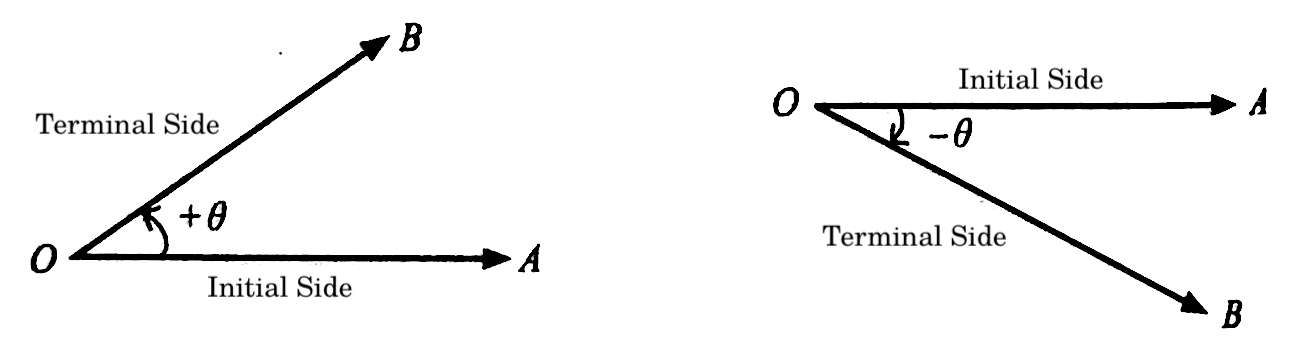
\includegraphics[scale=0.23]{assets/8-2.png}
\end{center}

\begin{explore}[Exploration Activity 1]
    
    \textbf{Aim:} To understand the definition of arbitrary angle.

    \textbf{Materials Needed:} A piece of paper, a protractor, a ruler

    \textbf{Steps:}
    \vspace{-1em}
    \begin{enumerate}
        \item Draw three parallel rays $OA$ (as shown below) on the paper. Hence, with $OA$ as the initial side of the angle, measure the following using a protractor:
        \begin{enumerate}
            \item The terminal side $OB$ of the $160^\circ$.
            \item The terminal side $OC$ of the $-45^\circ$.
            \item The terminal side $OD$ of the $450^\circ$.
        \end{enumerate}
        \item Write down clearly the respective direction and the measurement of the rotation in the three figures above.
    \end{enumerate}

    \textbf{Tool:} \underline{\url{https://www.geogebra.org/m/u7a3zxfd}}
\end{explore}

From exploration activity 1, this kind of directional rotational measurement that is not limited to $0^\circ$ to $360^\circ$ is known as the \textbf{arbitrary angle}. If the initial side doesn't rotate at all, the angle formed is called a \textbf{zero angle}.

\subsection*{Degree and Radian}

Back in junior high, the angle unit that we learned is formed by dividing a circle into $360$ equal parts, and the corresponding central angle of each part is known as 1 degree, denoted as $1^\circ$. Dividing the arc corresponding to 1 degree angle into $60$ equal parts, the corresponding central angle of each part is known as 1 minute, denoted as $1'$. Dividing the arc corresponding to 1 minute angle into $60$ equal parts, the corresponding central angle of each part is known as 1 second, denoted as $1''$.
\begin{align*}
    \therefore 1 \text{ full angle} & = 360^\circ\\
    1^\circ & = 60'\\
    1' & = 60''
\end{align*}
This form of base 60 measurement of angles is known as the \textbf{degree measure}.

\begin{explore}[Exploration Activity 2]

    \begin{enumerate}[label=\textbf{Aim:} ,leftmargin=4.5em]
        \item To inspect the relationship between arc length and radius, and to understand teh definition of radian measure.
    \end{enumerate}
    \vspace{-2em}
    \begin{enumerate}[label=\textbf{Materials Needed:} ,leftmargin=2em, align=left]
        \item A compass, a protractor, a string of length 10 cm, a scrap paper.
    \end{enumerate}
    \vspace{-1em}

    \textbf{Steps:}
    \vspace{-1em}
    \begin{enumerate}
        \item Form a group of 2 to 4 people, each group member is required to draw a circle with different radii. (Choose any arbitrary radius like 2cm, 3cm, 4cm, $\cdots$)
        
        \item Each person uses a line to measure the arc $AB$ with the same length as the radius on his own arc, then marks it on the string, as shown in the figure below.
        
        \begin{center}
            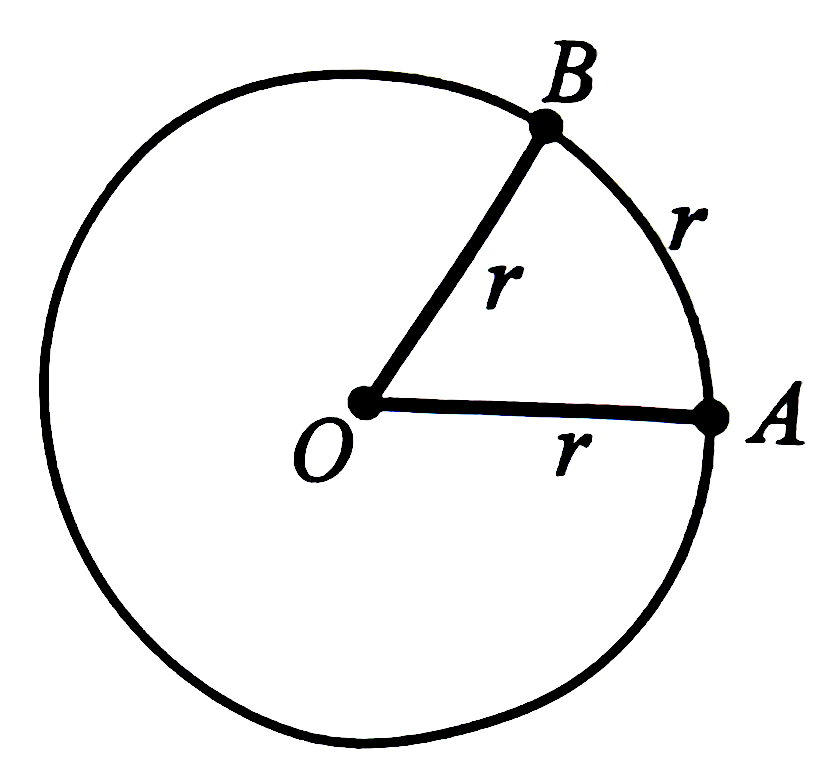
\includegraphics[scale=0.1]{assets/8-3.png}
        \end{center}
        
        \item Use a protractor to measure the corresponding central angle of the arc $AB$.
    \end{enumerate}

    \textbf{Discuss and Discover:}
    \vspace{-1em}
    \begin{enumerate}
        \item Compare the diagram drawn by each group member, are the measured central angles the same?
        \item Use a string to measure how many parts with the same length as the $AB$ of the circumference can be divided.
        \item Is it possible to derive an accurate answer for the question above using the formula of the circumference of a circle?
    \end{enumerate}
\end{explore}

From the activities above, we have led out another form of angle measurement that is commonly used in higher mathematics and other fields of science, known as the \textbf{radian measure}. We call the central angle corresponding to the arc with the same length as the radius (i.e. $\angle AOB$ in the figure above) 1 radian, denoted as $1 \text{ rad}$. From discussion 2 and discussion 3, we know that the ratio between the circumference of a circle and its radius is $2\pi$, i.e. 1 full angle $= 360^\circ = 2\pi \text{ rad}$, hence we can derive the following conversion formula between degree and radian:

\begin{align*}
    \pi \text{ rad} &= 180^\circ\\
    1 \text{ rad} &= \frac{180}{\pi}^\circ\\
    1^\circ &= \frac{\pi}{180} \text{ rad}
\end{align*}

\begin{question}
    Convert the following angles from degree to radian:
    \vspace{-1em}
    \begin{multicols}{2}
        \begin{enumerate}[label=(\alph*)]
            \item $218.84^\circ$
            \item $48^\circ 36'$
        \end{enumerate}
    \end{multicols}
    \vspace{-1em}
    \sol{}
    \begin{enumerate}[label=(\alph*)]
        \item \begin{align*}
            218.84^\circ &= 218.84 \times \frac{\pi}{180}\\
            &= 3.8195 \text{ rad}
        \end{align*}
        \item \begin{align*}
            48^\circ 36' &= \left(48 + \frac{36}{60}\right)^{\circ}\\
            & = 48.6 \times \frac{\pi}{180}\\
            & = 0.8482 \text{ rad}
        \end{align*}
    \end{enumerate}
\end{question}

\begin{question}
    Convert 1.5 radian to degree (accurate to minute).

    \sol{}
    \begin{align*}
        1.5 \text{ rad} &= 1.5 \times \frac{180}{\pi}^\circ\\
        &= 85^\circ 57'
    \end{align*}
\end{question}

\begin{question}
    Convert $\dfrac{\pi}{45}$ radian to degree.

    \sol{}
    \begin{align*}
        \frac{\pi}{45} \text{ rad} &= \frac{\pi}{45} \times \frac{180}{\pi}^\circ\\
        &= 4^\circ
    \end{align*}
\end{question}

It is worth nothing that when we use the radian measure, the unit "radian" is usually omitted. We usually write $90^\circ = \dfrac{\pi}{2}$, but if we use degree measure to express the same angle, the unit "degree" cannot be omitted.

\subsection*{\faFlag\ Practice 8.1 \xrfill[0.175\baselineskip]{1pt}} 

\begin{enumerate}
    \item Complete the following table, express the angle in $pi$:
    
    \begin{tabular}{|l|c|c|c|c|c|c|c|c|c|c|}
        \hline Angle & $0^{\circ}$ & $30^{\circ}$ & $45^{\circ}$ & $60^{\circ}$ & $90^{\circ}$ & $120^{\circ}$ & $135^{\circ}$ & $150^{\circ}$ & $180^{\circ}$ & $270^{\circ}$ \\
        \hline Radian & & & & & & & & & & \\
        \hline
        \end{tabular}

        \item Convert the following angles from radian to degree (if the result is not an integer, round to 2 decimal places):
        \vspace{-1em}
        \begin{multicols}{2}
            \begin{enumerate}[label=(\alph*)]
                \item $0.5 \text{ rad}$
                \item $\dfrac{7\pi}{6} \text{ rad}$
            \end{enumerate}
        \end{multicols}
\end{enumerate}

\subsection*{\faPencil\ Exercise 8.1 \xrfill[0.175\baselineskip]{1pt}}

\begin{enumerate}
    \item Using the horizontal ray $OA$ in the figure below as the initial side, sketch the position of the terminal side $OB$ of the following angles:
    \begin{center}
        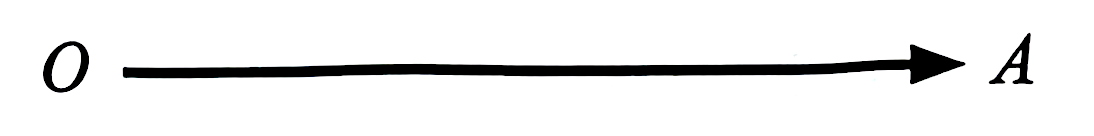
\includegraphics[scale=0.15]{assets/8-4.png}
    \end{center}
    \vspace{-1em}
    \begin{multicols}{3}
        \begin{enumerate}[label=(\alph*)]
            \item $\dfrac{5 \pi}{4}$
            \item $-\dfrac{6 \pi}{7}$
            \item $\dfrac{5 \pi}{2}$
        \end{enumerate}
    \end{multicols}
    
    \item Convert the following angles from degree to radian (accurate to 4 decimal places):
    \vspace{-1em}
    \begin{multicols}{3}
        \begin{enumerate}[label=(\alph*)]
            \item $68^\circ 93'$
            \item $139^\circ 12'$
            \item $-502^\circ 46'$
        \end{enumerate}
    \end{multicols}

    \item Convert the following angles from radian to degree (if the result is not an integer, round to minute):
    \vspace{-1em}
    \begin{multicols}{3}
        \begin{enumerate}[label=(\alph*)]
            \item $0.89 \text{ rad}$
            \item $-\dfrac{17\pi}{4} \text{ rad}$
            \item $3 \text{ rad}$
        \end{enumerate}
    \end{multicols}

    \item If the gear in the figure below rotates counterclockwise about its origin $O$, how many radians does the gear rotate through such that
    \begin{center}
        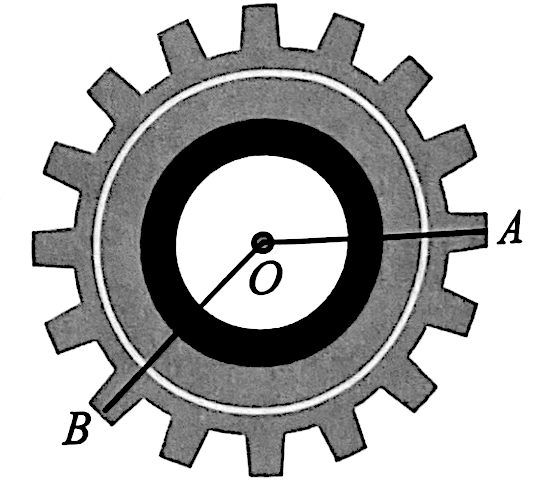
\includegraphics[scale=0.2]{assets/8-5.png}
    \end{center}
    \begin{enumerate}
        \item The line segment $OB$ reaches the position of $OA$ in the figure above for the first time?
        \item The line segment $OB$ reaches the position of $OA$ in the figure above for the second time?
    \end{enumerate}
\end{enumerate}

\end{document}
